
\section{Análise Semantica (\texttt{checker})} \label{section-checker}
processo de validação semântica no compilador é crucial para assegurar a corretude das equações, a consistência de tipos em operações e a resolução adequada de símbolos. Ele é estruturado em dois mecanismos principais: validação de definições de funções e validação de declarações. Esses mecanismos trabalham de forma integrada para garantir que a estrutura do programa esteja em conformidade com as regras semânticas da \texttt{EquationLang}.

Nesta seção, abordamos essas regras e discutimos como são validadas expressões envolvendo vetores, redefinições de equações e possíveis erros nas definições de BRDFs que inviabilizem a geração de código. A conclusão bem-sucedida dessa etapa de inferência e validação indica que o programa está apto a prosseguir para a fase de geração de código GLSL, conduzida pelo pacote \texttt{emitter}.


\subsection{Funções do Pacote \texttt{checker}}

O pacote \texttt{checker} é responsável por realizar diversas tarefas fundamentais para a validação semântica do compilador. Essas tarefas são descritas detalhadamente a seguir:

\begin{enumerate}
    \item \textbf{Inferência e Anotação de Tipos}:
    Cada expressão na AST possui um campo \verb"ty_inferred" que deve ser preenchido durante essa etapa. Para determinar esses tipos, é necessário realizar a inferência de tipos. Essa tarefa é detalhada na \autoref{subsection-type-inference}. Os tipos possíveis incluem números (\verb"float"), vetores (\verb"vector") e funções.
        O tipo de uma função é representada por um domínio (tipos dos argumentos de entrada) e um contradomínio (tipo do valor de retorno). Exemplos incluem:
        \begin{itemize}
            \item Uma função $f(a, b) = a \cdot b \cdot \vec{1,1,1}$, que recebe dois valores reais e retorna um vetor tridimensional, possui a assinatura:
            \[
            f : \mathbb{R} \times \mathbb{R} \to \mathbb{R}^3.
            \]
            \item O produto vetorial, que combina dois vetores tridimensionais, possui a assinatura:
            \[
            \times : \mathbb{R}^3 \times \mathbb{R}^3 \to \mathbb{R}^3.
            \]
        \end{itemize}
        Essas assinaturas são coletadas durante o processo de inferência para garantir a consistência em expressões de chamada de funções.

    \item \textbf{Compatibilidade de Tipos}:
    O \texttt{checker} também verifica a compatibilidade entre tipos em diferentes contextos do programa. Essa validação assegura que:
    \begin{itemize}
        \item Não sejam realizadas operações não definidas por \texttt{EquationLang}, como a multiplicação entre dois vetores. Por exemplo, $\vec{u} * \vec{v}$ seria inválido para uma multiplicação direta, mas pode ser válido para um produto escalar ou vetorial.

        \item Não sejam aplicados operadores em tipos incompatíveis, como elevar um número a um vetor ($2^{\vec{n}}$).

        \item Os argumentos de uma função pertençam ao domínio da função. Por exemplo, se a função $\texttt{normalize}(\vec{u})$ retorna um vetor tridimensional ($\mathbb{R}^3$), usá-lo como argumento para funlção seno, que espera um número escalar ($\mathbb{R}$). Então, $\sin(\texttt{normalize}(\vec{u}))$ seria inválido.
        \item O tipo do valor de retorno de uma função seja adequado ao contexto onde é utilizado.
    \end{itemize}

    \item \textbf{Validação de Definições de Símbolos}:
        Outro papel fundamental do \texttt{checker} é garantir que todos os identificadores, abstraido em símbolos na \autoref{subsection-symbols-scopes}, utilizados no programa estejam devidamente definidos antes de serem usados. Essa etapa inclui:
    \begin{itemize}
        \item Identificar declarações ausentes.
        \item Identificar dependencia circular.
        \item Certificar-se de que funções obrigatórias, como a BRDF $f$, estejam presentes.
    \end{itemize}
\end{enumerate}

Essas validações são realizadas utilizando o padrão \textit{Visitor}, detalhado na \autoref{subsection-walker} e os erros encontrados são reportados usando as funções de erros introduzida na \autoref{section-lexer} (\label{function-errors}).

\subsection{Uso do Padrão Visitor}
@@@ Prefisamos manter essa subseção se já vamos detalhar mais pra frente?@@

Para realizar a validação semântica, o pacote \texttt{walker} é reutilizado, permitindo a travessia modular da AST. Essa abordagem facilita a aplicação recursiva de inferência de tipos, provida pelo, mesmo em expressões aninhadas.

Validações ocorrem nessa traversia e basedo no tipo do nó, a inferencia é feita, discutido na \autoref{subsection-inferencia-tipos} uma operação binária de multiplicação:
\begin{itemize}
    \item Se ambos os operandos forem números reais, o resultado também será um número real.
    \item Se um dos operandos for um vetor tridimensional, o resultado dependerá do outro operando (por exemplo, um escalar ou outro vetor).
\end{itemize}

Como a esquerda ou a direita de uma operação binária podem ser expressões aninhadas (outras operações binárias, chamadas de funções, etc.), o padrão visitor permite aplicar a inferência de tipos recursivamente. Esse processo garante que o tipo de cada subexpressão seja determinado de forma consistente e confiável.


\subsection{Tipos, Simbolos e Escopos} \label{subsection-symbols-scopes}

Cada expressão na AST possui um tipo associado, modelado como uma união de estruturas na linguagem Odin, conforme mostrado na \autoref{cod-types-structs}. Essa abordagem permite representar diferentes categorias semânticas, como: tipos primitivos fundamentais, como números e vetores. assinaturas de funções, que capturam o domínio e o contradomínio. Por exemplo, o produto vetorial possui a assinatura $\mathbb{R}^3 \times \mathbb{R}^3 \to \mathbb{R}^3$. Já o vetor normal ($\vec{n}$), possui tipo primitivo de número ($\mathbb{R}$). A modelagem clara de tipos e o conceito de escopos e símbolos é essencial para validar expressões em diferentes contextos, verificar compatibilidade de operações e garantir a consistência semântica do programa.


\subsubsection{Tipos}
No \autoref{cod-types-structs}, temos a representação de tipos segue uma modelagem hierárquica o \textbf{Tipo Base} contém metadados comuns
como referência ao nó na arvóre sintática, identificador de tipo concreto. Os \textbf{Tipos Derivados} são enumerados a seguir:

\begin{enumerate}
    \item \textit{Tipo Básico:} Categorização primitiva (número)
    \item \textit{Tipo Vetorial:}
    \begin{itemize}
        \item Dimensionalidade
        \item Tipo de elemento
    \end{itemize}
    \item \textit{Tipo Funcional:}
    \begin{itemize}
        \item Parâmetros
        \item Resultados
    \end{itemize}
\end{enumerate}

\begin{codigo}[htb]
    \caption{\small Estruturas que representam o tipo de um expressão da AST. }
    \label{cod-types-structs}
\begin{lstlisting}[language=C, numbers=none, frame=none, inputencoding=latin1]

Type :: struct {
    node:    ^Node,
    size:    i64,
    derived: Any_Type,

    /* Easy comparison, types aren't equal if they are not even the same odin typeid */
    id:      typeid,
}

Type_Vector :: struct {
    using _:      Type,
    element_type: ^Type,
    dimensions:   int,
}


Type_Basic :: struct {
    using _: Type,
    basic_kind : Basic_Kind,
};


Type_Function :: struct {
    using _: Type,
    // node:   ^Expr_Procedure,
    params, results :[]^Type,
};

\end{lstlisting}
\end{codigo}


\subsubsection{Gerenciamento de Símbolos}

Os símbolos representam entidades nomeadas em \texttt{EquationLang}. A estrutura \texttt{Symbol}, apresentada no \autoref{cod-symbol}, encapsula as informações semânticas necessárias sobre os identificadores para validação da AST e geração de código. Essas informações incluem: \begin{itemize} \item \textbf{Escopo}: o escopo em que o símbolo foi definido. \item \textbf{Nó do identificador}: referência ao nó correspondente na AST para uso futuro. \item \textbf{Definição de função (opcional)}: nó da definição de função, quando aplicável. \item \textbf{Estado de resolução}: indica se o símbolo já foi resolvido. \item \textbf{Tipo associado}: o tipo inferido ou declarado do símbolo. \end{itemize}

O gerenciamento de símbolos é essencial para garantir que o estado de cada símbolo seja mantido durante a resolução, como discutido na \autoref{sec-symbol-resolution}.
\begin{enumerate}
    \item \textbf{Não Resolvido:} Estado inicial
    \item \textbf{Em Progresso:} Resolução em andamento
    \item \textbf{Resolvido:} Completamente processado
\end{enumerate}

\begin{codigo}[htb]
    \caption{\small Esturura do Simbolo. }
    \label{cod-symbol}
\begin{lstlisting}[language=C, numbers=none, frame=none, inputencoding=latin1]
// An Symbol is a named entity in the language
Symbol :: struct  {
    scope:      ^Scope,

    identifier: ^ast.Expr_Identifier, // Can be nullptr
    fn_defn:    ^ast.Expr_Function_Definition, // if the Symbol is a function

    state:      Symbol_State,
    flags:      bit_set[Symbol_Flag; u64],
    type:       ^Type,
    value:      Maybe(Value)
};

\end{lstlisting}
\end{codigo}


\subsection{Tabela de Símbolos}

Nesse projeto, foi desenvolvido também uma tabela de símbolos, cuja implementação é usada análise semântica e na geração de código GLSL. A implementação da tabela de símbolos fornecida aqui é baseada em uma estrutura de escopo hierárquico, onde cada escopo mantém um mapeamento entre os nomes dos símbolos e seus atributos correspondentes. No \autoref{struct-symbol}, a estrutura \texttt{Scope} representa um mapeamento de nomes para objetos de símbolo dentro de um \textbf{único escopo}, e a estrutura \texttt{Scope\_Table} mantém uma \textbf{pilha de escopos}, permitindo aninhamento.

\begin{codigo}[H]
\caption{\small Código da estrutura de símbolos escrito em Odin.}
\label{struct-symbol}
\begin{lstlisting}[language=C]
Scope_Table :: [dynamic]^Scope

SCOPES := Scope_Table{}

Scope :: struct {
/*
 . `node` Is a parent node that created that scope
 . Ex: a block, a function block, a struct or namespace
 . If null, then the scope is the file/global idk yet @LOOK
*/
    parent:   ^Scope,
    children:   [dynamic]^Scope,
    /*
     . It does not need to be a pointer to a map
     . because we don't ever copy a Scope we have only one scope
     . per map elements, and we access this ONLY scope value trought a pointer
    */

    elements: map[string]^Symbol,
    ordered_keys: []string, // bit of a HACK, yeah
};

\end{lstlisting}
\end{codigo}


\subsubsection{Gerenciamento de Escopo}

A tabela de símbolos fornece funções para gerenciar escopos, incluindo:
\begin{itemize}
    \item \texttt{scope\_enter}: entrar em um novo escopo, anexando-o à pilha de escopos.
    \item \texttt{scope\_exit}: sai do escopo atual, removendo-o da pilha de escopos e o retornando.
    \item \texttt{scope\_reset}: redefine a tabela de símbolos limpando todos os escopos.
    \item \texttt{scope\_get}: recupera um símbolo da tabela de símbolos pelo seu identificador.
    \item \texttt{scope\_add}: adiciona um novo símbolo ao escopo atual.
\end{itemize}

Essa tabela de símbolos armazena todas as informações necessárias para a fase de geração do \textit{shader} GLSL.


\subsubsection{Resolução de Símbolos}

A resolução de símbolos é uma etapa fundamental no \texttt{checker}, garantindo que cada símbolo seja corretamente definido e tipado antes de seu uso. Esse processo é especialmente relevante em situações onde a ordem de definição não segue um fluxo linear. Por exemplo:

\[
b = a
\]

\[
a = \vec{1, 0, 1}
\]

Nesse caso, \texttt{b} é atribuído a \texttt{a} antes que \texttt{a} tenha sido definido. O \texttt{checker} deve resolver essa dependência, analisando \texttt{a} antes de \texttt{b} para inferir corretamente o tipo de \texttt{b}. Isso é possível por conta da construção de um grafo de dependências entre símbolos (apresentado na \autoref{cod-grafo-simbol-deps}). Utilizando uma ordenação topológica desse grafo, o sistema determina uma ordem de avaliação válida, além de identificar ciclos de dependência, como em casos de dependências circulares que poderiam impedir a compilação.

Essa abordagem permite o uso de simbolos antes da sua equação ser declarada, desde que estejam devidamente definidas em alguma das equações. Adicionalmente, a resolução de símbolos lida com escopos, parâmetros de funções e símbolos embutidos, que são os definidos na tabela de convenções de símbolos matemáticos (\autoref{@va trabahlhar vagabundo@}). A resolução de simbolos gera um ordem correta de avaliação das declaraçãos, recurso particularmente importante na geração de código GLSL, onde referências a variáveis antes de suas declarações não são permitidas. A resolução de simbolo considera o escopo do simbolo apropriadamente e nessa etapa que detectamos se a função $f$, a BRDF por convenção, existe no escopo global. Para implementar essas funcionalidades, o pacote \texttt{checker} é dividido em múltiplas passadas na AST:

\begin{enumerate}
    \item \textbf{Coleta de Símbolos}:
    \begin{itemize}
        \item Reunir todas as declarações
        \item Registrar símbolos nos escopos apropriados
        \item Inicializar estruturas de rastreamento de dependências
    \end{itemize}

    \item \textbf{Análise de Dependências}:
    \begin{itemize}
        \item Construir o grafo de dependências
        \item Validar referências de símbolos; inclue detectar uso de simbolos que nunca foram definidas.
        \item Estabelecer a ordem de avaliação
    \end{itemize}

    \item \textbf{Validação Final}:
    \begin{itemize}
        \item Inferencia e verificação de tipos
        \item Verificação do ponto de entrada
        \item Validação de definição de funções com uso escopo
    \end{itemize}
\end{enumerate}



% Cosegue lidar com escopo, parametros de funções e simbolos embutidos, aqueles padrões dinifidos na tabela de convenções de simbolos matematiccos \autoref{@va trabahlhar vagabundo@}. Para isso exist multiplas passadas. A primeira coleta todos os simbolos. A segunda, analisa as dependencias e estabelece a ordem de avaliação. Por ultimo, o \texttt{checker} toma contra do restante das inferencias de tipos e outras validações

\begin{codigo}[htb]
    \caption{\small Entrada para o compilador que gera dependencia circular. }
    \label{cod-grafo-simbol-deps}
\begin{lstlisting}[language=C, numbers=none, frame=none, inputencoding=latin1]
\begin{equation}
    a = f
\end{equation}

\begin{equation}
    f = a
\end{equation}

\end{lstlisting}
\end{codigo}

\begin{figure}[H]
    \caption{\label{label} \small Erro reportado sobre dependencia circular.}
    \begin{center}
        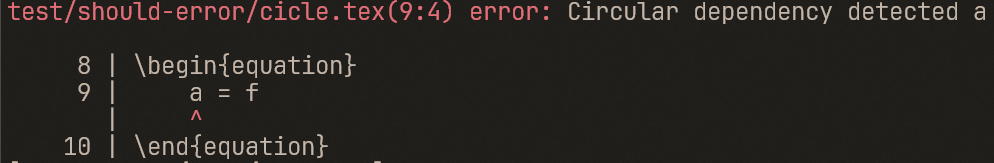
\includegraphics[scale=0.5]{./Imagens/error-circular-deps.png}
    \end{center}
\end{figure}


\subsection{Inferencia de Tipos} \label{subsection-inferencia-tipos}


A função \verb`infer_type` serve para determinar o tipo de uma expressão sintática (representada por \verb`expr`) em uma árvore abstrata (AST) durante a análise semântica. É usado um conjunto de regras e verificações para inferir e atribuir tipos a expressões com base nas regras matematicas como multiplicação entre numero real e vetor, produtor vetorial dentre dois vetores, assinatura de funções definidas, etc.  Essa função é projetada para lidar com diversas construções que são expressões, como identificadores, operadores prefixados e infixados, chamadas de função e literais.



Inicialmente, a função verifica se o tipo da expressão já foi inferido (\verb"expr.ty_inferred"). Se sim, retorna o tipo previamente inferido, evitando processamento redundante. Caso contrário, prossegue com a inferência.

O bloco central da função é um \verb"switch" que analisa os diferentes tipos de expressões derivadas de \verb"expr". Um trecho relevante dessa implementação está no \autoref{cod-type-inference}.

Para \textbf{identificadores} (\verb"Expr_Identifier"), verifica se o identificador corresponde a um vetor especial, como $\omega_i$ ou $\vec{v}$. Nesse caso, o tipo é inferido como $\mathbb{R}^3$ (vetor tridimensional). Identificadores específicos, como \verb"\pi" ou \verb"\epsilon", são atribuídos ao tipo numérico real ($\mathbb{R}$). Para outros identificadores, a função consulta o escopo atual para determinar o tipo, usando as estruturas detalhado na sessão \autoref{@@@@@@}. Caso o identificador não seja encontrado, a função reporta um erro.

\begin{codigo}[htb]
    \caption{\small Parte do switch da inferencia de tipos. }
    \label{cod-type-inference}
\begin{lstlisting}[language=C, frame=none, inputencoding=utf8]
infer_type :: proc(expr: ^ast.Expr, allow_invalid := false, default : ^ast.Type = ast.ty_invalid ) -> ^Type {
    /// Código omitido por brevidade  ///
    #partial switch e in expr.derived {
    case ^Expr_Identifier:
        // Alway set by the parser if indentifier starts with `\vec{}`
        if e.is_vector {
            type = new_type_vector(ty_number, 3) // vector 3 of type number (real)
        } else if e.identifier.kind == .Pi || e.identifier.kind == .Epsilon {
            type = ty_number
        } else {
            key := key_from_identifier(e)
            sym, ok := scope_get(key)
            if ok {
                if sym.type != nil {
                    type = sym.type
                }
            }
            /// Código omitido por brevidade  ///
        }

    case ^Expr_Prefix:
        right_type := infer_type(e.right, allow_invalid, default)
        /// Código omitido, mas aqui fazemos a validação da subexpressão direita e atribuimos o tipo correto para Expr_Prefix   ///

    case ^Expr_Infix:
        ty_left  := infer_type(e.left, allow_invalid, default)
        ty_right := infer_type(e.right, allow_invalid, default)
        /// Código omitido
        //  Inferimos tipo da expressão esquerda e direto dessa operação binária
        //  Depois validamos compatibilidade considerando a operação sendo usada nessas duas expressões

    /// Outros casos ...  ///
}
\end{lstlisting}
\end{codigo}


Para \textbf{operações prefixadas} (\verb"Expr_Prefix"), como raiz quadrada (\verb"\sqrt") ou funções trigonométricas (\verb"\sin", \verb"\cos"), a função valida se o operando é numérico e atribui o tipo correspondente à expressão. Nas \textbf{operações binárias} (\verb"Expr_Infix"), a função realiza a inferência dos tipos dos operandos esquerdo e direito. Se os tipos não forem compatíveis, aplica regras específicas. Alguma dessas regras são:

\begin{itemize}
    \item A multiplicação de um número por um vetor ($2*\vec{n}$) ou a divisão de um vetor por um número ($\frac{\vec{u}}{\sqrt{\vec{u} \cdot \vec{u}}}$) resultam no tipo vetor ($\mathbb{R}^3$).
    \item Operações entre dois vetores ou dois números seguem as regras padrão associadas ao operador.
\end{itemize}

Outros casos incluem \textbf{literais}, como números (\verb"Expr_Number") e vetores literais (\verb"Expr_Vector_Literal"), cujos tipos são atribuídos diretamente como $\mathbb{R}$ (números reais) e $\mathbb{R}^3$ (vetores tridimensionais), respectivamente.



Para chamadas de função (\verb"Expr_Function_Call"), o tipo da expressão é determinado pelo tipo do primeiro valor retornado pela função. A validação dos argumentos é realizada em outra função, detalhada na sessão @@@. Erros encontrados são reportados com mensagens detalhadas, como descrito na \autoref{subsection-erros}.

% ; Essa parte já foi dita
% Além disso, a função realiza validações específicas para evitar inconsistências, como garantir que operações entre vetores sejam semanticamente válidas (e.g., divisão entre vetores não é permitida). 

% Em resumo, \verb`infer_type` é uma implementação robusta e flexível de inferência de tipos, essencial para a análise semântica de um compilador. A função assegura que cada expressão receba um tipo coerente com a semântica da linguagem, lidando com uma ampla gama de construções sintáticas e oferecendo suporte extensível para futuras adições à linguagem.


\subsection{Tipos de Expressões}

\subsubsection{Validação de Funções}
A validação semântica de definições e chamadas de funções segue um processo semelhante ao da análise de expressões, mas o uso da pilha de escopos. As variáveis no corpo da função (lado direito da equação) devem ser validadas para garantir que todos os símbolos estejam definidos.

A validação do corpo da função representa a etapa final do processo de checagem e envolve:

\begin{enumerate}
    \item Validar todas as expressões no corpo da função.
    \item Inferir o tipo de retorno com base na expressão final.
    \item Construir o tipo completo da função, incluindo parâmetros e retorno.
    \item Garantir que todos os identificadores utilizados estejam consistentes com seus tipos declarados.
\end{enumerate}
%%%

O processo começa com o processamento dos parâmetros e o gerenciamento do escopo. Quando uma função é definida, o sistema cria um novo escopo para armazenar informações dos parâmetros e da própria função em forma de simbolos à serem adicionados ao escopo atrelado a essa definição.

Esse escopo com simbolos são essencial para validar tanto as chamadas de função quanto as expressões no corpo da função. Cada função tem seu próprio escopo, cujo escopo pai é o global, prevenindo conflitos de identificadores.

Na definição de escopo, se o $x$ existe nos parâmetros, primeiro é usado o $x$ do parâmetro antes de tentar acessar um $x$ global. Isso é chamado de \textit{shadowing} ou sombreamento do símbolo, como no caso da equação \autoref{eq-shadowing}, o resultado de $f$ é 3 e não 2.

\begin{align} \label{eq-shadowing}
    &x = 2 \\
    &g(x) = x \\
    &f = g(3)
\end{align}


%%%
Durante a validação dos parâmetros, cada identificador passa pela inferência de tipo. Parâmetros explicitamente marcados com o prefixo \verb"\vec" recebem o tipo padrão $\mathbb{R}^3$ (vetor tridimensional). Caso contrário, o tipo padrão atribuído é o de número real ($\mathbb{R}$).

A validação de identificadores do corpo da função (lado direito da equação) usa o escopo da função para verificar se o identificador está definido, se seu tipo é compatível com o encontrado no simbolo presente neste escopo; e verifica ele não viola as regras semânticas.

Identificadores especiais, como $\omega_i$ e $\theta_d$, são inseridos automaticamente no escopo global com seus tipos predefinidos. Por exemplo, se o parâmetro $\vec{x}$ é declarado como vetor, todo uso de x no corpo da função deve respeitar as operações vetoriais, ou um erro será reportado.


Chamadas de função passam por uma validação semelhante: os argumentos fornecidos têm seus tipos inferidos e são comparados com a assinatura da função chamada (\verb"Type_Function"). Por exemplo, no código da \autoref{cod-type-mismatch}, a função $g$ tem a assinatura $\mathbb{R} \times \mathbb{R} \to \mathbb{R}$. A expressão de chamada de função resultante tem o tipo do contradomínio da função chamada. Se, por exemplo, $f$ espera dois números reais como argumentos e um vetor é passado no lugar de um deles, um erro será gerado. A \autoref{fig-type-mismatch} ilustra tal erro, indicando exatamente o argumento incompatível.

\begin{codigo}[htb]
    \caption{\small Equação com uso incorreto de tipos na chamada de função. }
    \label{cod-type-mismatch}
\begin{lstlisting}[language=tex, numbers=none, frame=none, inputencoding=latin1]
\begin{equation}
    g(a, x) = a*x*x
\end{equation}

\begin{equation}
    f = g(1, \vec{1,1,1})
\end{equation}

\end{lstlisting}
\end{codigo}

\begin{figure}[H]
    \caption{\label{fig-type-mismatch} \small Erro gerado por uso incorreto de tipos na chamada de função.}
    \begin{center}
        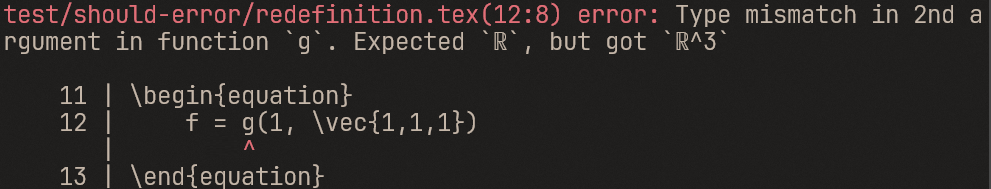
\includegraphics[scale=0.5]{./Imagens/error-type-mismatch.png}
    \end{center}
\end{figure}

\subsection{Validação de Equaçoes}

Para todos os identificadores, é criado um escopo global contendo todos os símbolos definidos. Declarações de equações são validadas verificando o lado esquerdo (LHS) das expressões, assegurando que o identificador esteja previamente definido. Isso ocorre após a etapa de coleta e ordenação descrita em \autoref{colega e ordenação de equações}. Cada LHS deve ser um identificador válido ou a definição de uma função. Esse processo também verifica redefinições de símbolos, prevenindo múltiplas declarações do mesmo identificador no mesmo escopo.

Todas as violações semânticas, como incompatibilidades de tipos ou uso de valores escalares onde vetores são esperados, são reportadas ao usuário, juntamente com informações detalhadas sobre o contexto e o local do erro.

Essa etapa de validação semântica provê a base necessária para garantir a correção do programa gerado, sendo crucial para a próxima etapa, que é a geração de código.

A função \verb"check_expr" realiza a mesma traversia que a interencia de tipos das expressões. Mas dessa vez fazendo validações que \texttt{infer\_type} deixou de fazer, garantindo que todas sigam as regras e sintaxe estabelecidas pela linguagem.

Os identificadores embutidos, definidos pelas convenções deste trabalho, são adicionados automaticamente à tabela de símbolos e estão prontos para uso imediato. A lista de identificadores embutidos pode ser vista em \autoref{cod-builtins}.

\begin{codigo}[htb]
    \caption{\small Identificadores embutidos pela convenção deste trabalho. }
    \label{cod-builtins}
\begin{lstlisting}[language=C, numbers=none, frame=none, inputencoding=latin1]
BUILTIN_IDENTIFIERS :: []string {
    `\max`,
    `\pi`,
    `\epsilon`,
    `\theta{h}`,
    `\vec{n}`,
    `\vec{h}`,
    `\vec{\omega{i}}`,
    `\theta{i}`,
    `\phi{i}`,
    `\vec{\omega{o}}`,
    `\theta{o}`,
    `\phi{o}`,
    `\theta{h}`,
    `\theta{d}`,
}
\end{lstlisting}
\end{codigo}


\subsubsection{Casos mais relevantes}

@Do we needs this again?@
\begin{itemize}
    
    \item Identificadores (\verb`Expr_Identifier`):
      Verifica se o identificador está definido no escopo atual. Caso contrário, gera um erro com a mensagem apropriada. Se estiver definido:
    \item **Chamadas de Função (\verb`Expr_Function_Call`)**: 
      A função realiza várias validações:
      - Verifica se a expressão da esquerda é um identificador válido.
      - Confirma que o identificador refere-se a um símbolo do tipo função.
      - Garante que o número e os tipos dos argumentos correspondem aos parâmetros esperados.
      - Para cada argumento, chama recursivamente \verb`check_expr`.
    \item **Expressões com Prefixo (\verb`Expr_Prefix`)**:  
      Avalia operadores como \verb`-`, \verb`+`, ou funções como `sqrt()` e `sin()`. Por exemplo:
      - Em \verb`sqrt(x)`, verifica se `x` é um número (\verb`ty_number`). Caso contrário, exibe um erro.
      - Para operadores básicos como \verb`-` e `+`, a inferência de tipo já determina o comportamento correto.
    \item **Literais de Vetor (\verb`Expr_Vector_Literal`)**:  
      Verifica se o vetor tem exatamente 3 dimensões. Caso contrário, gera um erro indicando o formato esperado.
\end{itemize}





\begin{codigo}[htb]
    \caption{\small Validação de parametros de uma função. }
    \label{cod-parametros-validation}
\begin{lstlisting}[language=C, numbers=none, frame=none, inputencoding=latin1]
// ...
parameter_types := [dynamic]^Type{}
scope_enter(fn_sym.scope) {
    for &parameter in fn.parameters {
        parameter_key := key_from_identifier(parameter)
        ty := infer_type(parameter, true, ty_number)
        parameter_sym.type = ty
        append(&parameter_types, ty)
    }
}
// ...
\end{lstlisting}
\end{codigo}


\begin{codigo}[htb]
    \caption{\small Validação de um uníco identificador. }
    \label{cod-check-single-ident}
\begin{lstlisting}[language=C, numbers=none, frame=none, inputencoding=latin1]

check_single_identifier :: proc(parameters: []^ast.Expr_Identifier, ident: ^ast.Expr_Identifier) {
    infer_type(ident)
    ident_key := key_from_identifier(ident)
    // Validates type consistency between declaration and usage
    if !is_type_equal(ident.ty_inferred, p.ty_inferred) {
        error(ident.identifier, "Parameter `%v` being use as type `%v` when the expected type is `%v`", ...)
    }
    // Código omitido por brevidade ..
}
\end{lstlisting}
\end{codigo}


% \subsection{Validação de Definição e Declaração de Função na Análise Semântica}

\subsection{Validação da Definição de Função}
O procedimento \verb`check_function_definition` implementa um sistema de validação abrangente para definições de função, garantindo segurança de tipos e consistência de parâmetros.

\subsubsection{Fase 1: Processamento de Parâmetros}
Aspectos principais:
\begin{itemize}
    \item Cria um novo escopo para os parâmetros da função
    \item Inferência de tipos para cada parâmetro
    \item Mantém informações sobre o tipo dos parâmetros
    \item Tratamento de tipo padrão (número se não for vetor)
\end{itemize}

\subsubsection{Fase 2: Validação de Identificadores}
Assim como no parser, temos uma correspondência entre os tipos da árvore sintática com \verb|Expr_Identifier|, \verb|Expr_Infix|, etc., com funções que podem ser indiretamente recursivas, como \verb|check_single_identifier| (\autoref{cod-check-single-ident}), \verb|check_expr|, etc.

\subsubsection{Fase 3: Validação do Corpo da Função}
\begin{codigo}[htb]
    \caption{\small Validação do corpo da função.}
    \label{cod-function-body-validation}
\begin{lstlisting}[language=C, numbers=none, frame=none, inputencoding=latin1]
scope_enter(fn_sym.scope) {
    check_expr(body)
    body_type := infer_type(body)
    result_types := [dynamic]^Type{body_type}
    fn_type := make_function_type(parameter_types[:], result_types[:])
}
\end{lstlisting}
\end{codigo}

Passos principais:
\begin{itemize}
    \item Validação de expressões
    \item Inferência do tipo de retorno
    \item Construção do tipo de função
    \item Gerenciamento de escopo
\end{itemize}

\subsection{Tratamento de Declaração de Equação}
\begin{codigo}[htb]
    \caption{\small Tratamento de declaração de equação.}
    \label{cod-equation-declaration}
\begin{lstlisting}[language=C, numbers=none, frame=none, inputencoding=latin1]
case ^Decl_Equation:
    check_decl(s)
\end{lstlisting}
\end{codigo}

\subsection{Mecanismos de Segurança de Tipos}
A implementação garante segurança de tipos através de vários mecanismos:

\begin{itemize}
    \item \textbf{Validação de Tipo de Parâmetro}
    \begin{itemize}
        \item Verificação explícita de tipos para parâmetros
        \item Tratamento de tipo vetor (reconhecimento do prefixo \verb|\vec|)
        \item Atribuição de tipo padrão
    \end{itemize}

    \item \textbf{Validação Baseada em Escopo}
    \begin{itemize}
        \item Gerenciamento hierárquico de escopo
        \item Controle de visibilidade de símbolos
        \item Isolamento de escopo de parâmetros
    \end{itemize}

    \item \textbf{Detecção de Erros}
    \begin{itemize}
        \item Detecção de incompatibilidade de tipos
        \item Validação de uso de parâmetros
        \item Verificação de violação de escopo
    \end{itemize}
\end{itemize}

\subsection{Detalhes Técnicos da Implementação}

\subsubsection{Resolução de Símbolos}
\begin{itemize}
    \item Símbolos de parâmetros são resolvidos dentro do escopo da função
    \item Inferência de tipos é realizada para todos os identificadores
    \item Consistência de tipos é aplicada em todo o corpo da função
\end{itemize}

\subsubsection{Gerenciamento de Escopo}
\begin{codigo}[htb]
    \caption{\small Gerenciamento de escopo na validação do corpo da função.}
    \label{cod-scope-management}
\begin{lstlisting}[language=C, numbers=none, frame=none, inputencoding=latin1]
scope_enter(fn_sym.scope) {
    // Validação do corpo da função
    check_expr(body)
    // Inferência e validação de tipo
    body_type := infer_type(body)
}
\end{lstlisting}
\end{codigo}
\section*{Validação de Campo de Declaração e Definição de Funções na Análise Semântica}

Este documento descreve o funcionamento das funções \texttt{check\_field} e \texttt{check\_function\_definition}, incluindo a validação semântica de campos, declaração de equações e definições de funções. 

\subsection*{Fluxo Geral da Função \texttt{check\_field}}

A função \texttt{check\_field} garante que os campos de uma estrutura ou declaração estejam semanticamente corretos. Esse processo segue as etapas abaixo:

\begin{itemize}
  \item \textbf{Validação do LHS (Chave):}  
  O lado esquerdo deve ser um identificador ou definição de função. Erros de validação são detalhados com mensagens explicativas.

  \item \textbf{Definições de Função:}  
  Chaves que representam definições de função são delegadas à função \texttt{check\_function\_definition}, que valida os parâmetros e o corpo da função.

  \item \textbf{Validação do RHS (Valor):}  
  O valor (\texttt{field.value}) é verificado recursivamente com \texttt{check\_expr}. Caso o tipo não esteja inferido, a inferência é realizada.

  \item \textbf{Comparação de Tipos:}  
  Após a inferência, verifica se os tipos do LHS e RHS são compatíveis. Inconsistências são detalhadas nas mensagens de erro.

  \item \textbf{Gerenciamento de Símbolos:}  
  Os símbolos representam variáveis ou funções na linguagem. Caso o símbolo já exista, ele é atualizado; caso contrário, um novo símbolo é criado.
\end{itemize}

\subsection*{Validação de Definições de Funções}

A função \texttt{check\_function\_definition} é responsável pela validação completa de definições de funções. Ela assegura a consistência dos parâmetros e a segurança de tipos.

\subsubsection*{Fase 1: Processamento de Parâmetros}
\begin{itemize}
  \item Cria um novo escopo para os parâmetros da função.
  \item Realiza inferência de tipos para cada parâmetro.
  \item Lida com tipos padrão (e.g., vetor para prefixos \textbackslash{}vec).
\end{itemize}

\subsubsection*{Fase 2: Validação do Identificador}
Correspondências entre a árvore sintática e os tipos são validadas recursivamente por funções como \texttt{check\_single\_identifier} e \texttt{check\_expr}.

\subsubsection*{Fase 3: Validação do Corpo da Função}
O corpo da função é validado em um escopo isolado:
\begin{itemize}
  \item Expressões são verificadas com \texttt{check\_expr}.
  \item O tipo de retorno é inferido e comparado com o tipo declarado.
  \item O tipo da função é construído com base nos parâmetros e resultados.
\end{itemize}

\begin{codigo}[htb]
    \caption{\small Estruturas que representam o tipo de um expressão da AST.}
    \label{cod-types-structs}
\begin{lstlisting}[language=C, numbers=none, frame=none, inputencoding=utf8]
case ^Decl_Equation:
    check_decl(s)

scope_enter(fn_sym.scope) {
    // Validação do corpo da função
    check_expr(body)
    // Inferência e validação de tipo
    body_type := infer_type(body)
    result_types := [dynamic]^Type{body_type}
    fn_type := make_function_type(parameter_types[:], result_types[:])
}
\end{lstlisting}
\end{codigo}

\subsection*{Mecanismos de Segurança de Tipos}

A implementação garante a segurança de tipos por meio de:
\begin{itemize}
  \item \textbf{Validação de Parâmetros:}
  Checagem explícita de tipos para parâmetros e reconhecimento de vetores (\textbackslash{}vec).

  \item \textbf{Gerenciamento de Escopos:}
  Uso de operações hierárquicas (\texttt{scope\_enter}/\texttt{scope\_exit}) para evitar conflitos de símbolos.

  \item \textbf{Detecção de Erros:}
  Identificação de inconsistências de tipo, violações de escopo e uso inválido de parâmetros.
\end{itemize}

\subsection*{Exemplo de Declaração de Equação}
